%\begin{multicols}{2}
Cette séance commencera par une présentation du fonctionnement d'un ordinateur (relative à la fin du chapitre 1 vu en cours). 
La seconde partie de la séance sera consacrée au TP en lui-même (Partie~\ref{sec.demontage}) : vous 
démonterez les anciens ordinateurs du lycée pour repérer et étudier leurs composants. 

\begin{enumerate}
\item  \textbf{Lisez attentivement  tout l'énoncé
    avant de commencer.}
\item Après la séance, vous devez rédiger un compte-rendu de TP et
l'envoyer au format électronique à votre enseignant.
\item Le seul format accepté pour l'envoi d'un texte de compte-rendu est le
format PDF. Votre fichier s'appellera impérativement \texttt{tp01\_durif\_pessoles.pdf}, où \og \texttt{durif}\fg\ et \og \texttt{pessoles}\fg\ sont à remplacer par les noms des membres du binôme. 
\item Ce TP est à faire en binôme, vous ne rendrez donc qu'un
  compte-rendu pour deux.
\item Pensez à vous munir d'un appareil photo (un smartphone est suffisant).
\item Avant d'envoyer le compte rendu, merci de vérifier que les photos incluses dedans sont d'un poids raisonnable.
\end{enumerate}

\section{Généralités sur le fonctionnement d'un ordinateur.}\label{sec.ordi}



\begin{exemple}[]
\textbf{Exemple ou contre-exemple d'ordinateur au sens de la définition apportée dans le cours ?}

\begin{minipage}{0.4\textwidth}
\begin{enumerate}
\item Automobile
\item Thermostat d'ambiance (mécanique)
\item Thermostat d'ambiance (électronique)
\item Téléphone portable (smartphone)
\item PC de bureau
\item Lecteur MP3
\item Box de votre FAI
\item Métier Jacquard
\end{enumerate}

\end{minipage}
\begin{minipage}{0.5\textwidth}
\begin{center}
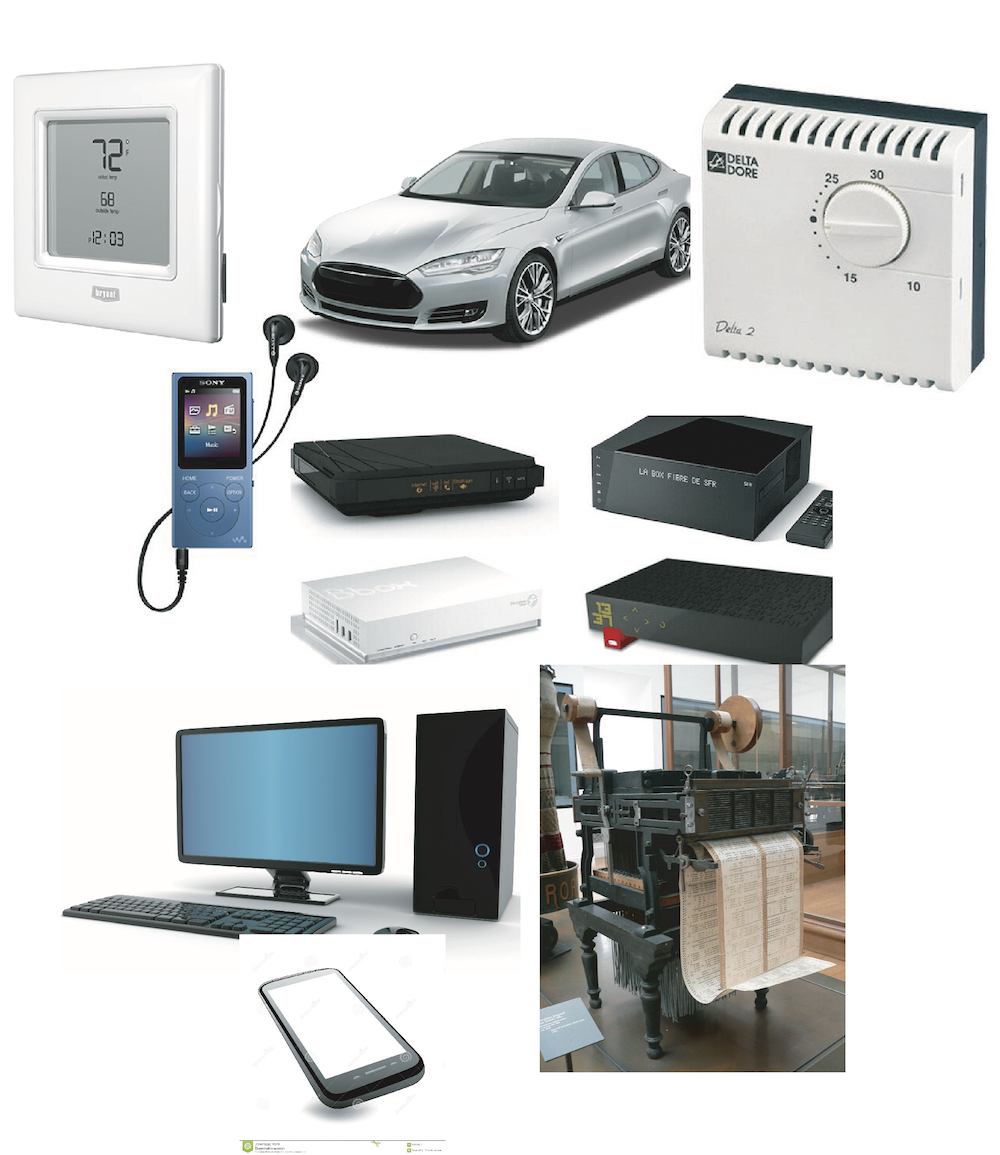
\includegraphics[width=0.7\textwidth]{montage_exemples.jpg}
\end{center}
\end{minipage}
\end{exemple}


\section{Démontage d'un PC et étude de ses composants.}\label{sec.demontage}

Avant tout, notez bien qu'on ne démonte pas les ordinateurs de la
salle de TP mais ceux fournis par l'enseignant dans ce but!

Deuxième chose : on ne touche pas l'intérieur du PC, ou alors le moins
possible et  en ayant pris  soin au préalable  de se décharger  de son
électricité statique en touchant la carcasse du PC.

Chaque  binôme  dispose  d'un PC.  Le  but  du  jeu est  de  l'ouvrir,
d'identifier  les différents  composants (où  est le  disque dur ? la
carte mère ? le processeur ?  la mémoire vive? ), puis de le refermer,
le tout sans casse.

N'oubliez pas de prendre des photos de l'intérieur pour votre
compte-rendu.

\emph{Vous préciserez sur le compte-rendu les différents éléments
  que vous avez identifiés, de préférence à partir de photos.}

\emph{Attention : vous ne démonterez pas ni la carte mère, ni le bloc d'alimentation électrique (vous pourrez ôter ce dernier du l'ordinateur).}  
%\end{multicols}